\documentclass{standalone}
\usepackage{tikz}
\usetikzlibrary{fit}
\usepackage[dvipsnames]{xcolor}
\usetikzlibrary{shapes.geometric}
\newcommand\x{4.5}
\begin{document}
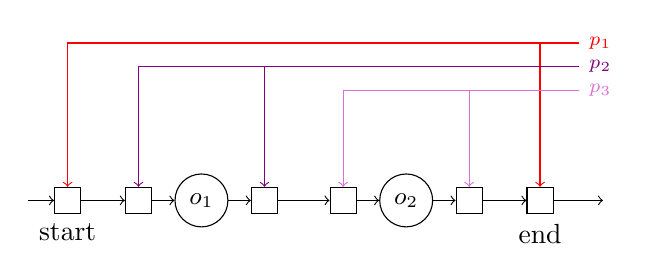
\begin{tikzpicture}[square/.style={regular polygon,regular polygon sides=4}, box/.style = {draw,red, dashed, inner sep=10pt,rounded corners=5pt}]
    \node at (-0.3,0) [circle, draw] (o1) {\small $o_1$};
    \node at (2.3,0) [circle, draw] (o2) {\small $o_2$};
    
    \node at (-1.1, 0) [square, minimum width = 0.2cm, draw] (s1) {};
    \node at (-2, 0) [square, minimum width = 0.2cm, draw, label = below:start] (sp) {};
    
    \node at (0.5, 0) [square, minimum width = 0.2cm, draw] (o1e) {};
    \node at (1.5, 0) [square, minimum width = 0.2cm, draw] (o2s) {};
    \node at (3.1, 0) [square, minimum width = 0.2cm, draw] (o2e) {};
    \node at (4, 0) [square, minimum width = 0.2cm, draw, label = below:end] (pe) {};
    

    \draw[->] (-2.5,0) -- (sp.west);
    \draw[->] (sp.east) -- (s1.west);
    \draw[->] (s1.east) -- (o1.west);
    \draw[->] (o1.east) -- (o1e.west);
    \draw[->] (o1e.east) -- (o2s.west);
    \draw[->] (o2s.east) -- (o2.west);
    \draw[->] (o2.east) -- (o2e.west);
    \draw[->] (o2e.east) -- (pe.west);

    \draw[->] (pe.east) -- (\x + 0.3, 0);

    %Probe 1
    \draw[->, red] (\x, 2) node[right] {\scriptsize $p_1$} -- (-2, 2) -- (sp.north) ;
    \draw[->, red] (4, 2) -- (pe.north);

    %Probe 2
    \draw[->, violet] (\x, 1.7) node[right] {\scriptsize$p_2$} -- (-1.1, 1.7) -- (s1.north);
    \draw[->, violet] (0.5, 1.7) -- (o1e.north);
    %Probe 3
    \draw[->, Orchid] (\x, 1.4) node[right] {\scriptsize $p_3$} -- (1.5, 1.4) -- (o2s.north);
    \draw[->, Orchid] (3.1, 1.4) -- (o2e.north);


\end{tikzpicture}
\end{document}

